\documentclass[12pt,a4paper]{report}
\usepackage[utf8]{inputenc} % un package
\usepackage[T1]{fontenc} % un second package
\usepackage[francais]{babel} % un troisième package
\usepackage{color} % Package de la couleur
\usepackage{verbatim}
\usepackage{moreverb}
\usepackage{amsmath}
\usepackage{amsfonts}
\usepackage{amssymb}
\usepackage{graphicx}
\usepackage[top=2cm, bottom=2cm, left=2cm, right=2cm]{geometry}
\author{IMA World Health Web Developer Team}
\title{
\includegraphics[width=12cm]{ima.png} \\Hospital Management System\\ (HMS) \\ Manuel d'utilisation}

\begin{document}
%Page de garde
\maketitle 
\chapter{Présentation}
\section{Accès au système}
\large{Pour accéder au système, la première de chose à faire est de lancer un navigateur web, en suite saisir l'adresse web de l'application dans la barre d'adresse du navigateur.}

La première interface de l'application est un formulaire qui demande à chaque utilisateur de pouvoir fournir le login, le mot de passe mais  aussi le projet dont il sont assigné, comme le montre le formulaire ci-dessous.
\begin{figure}[h]
\begin{center}
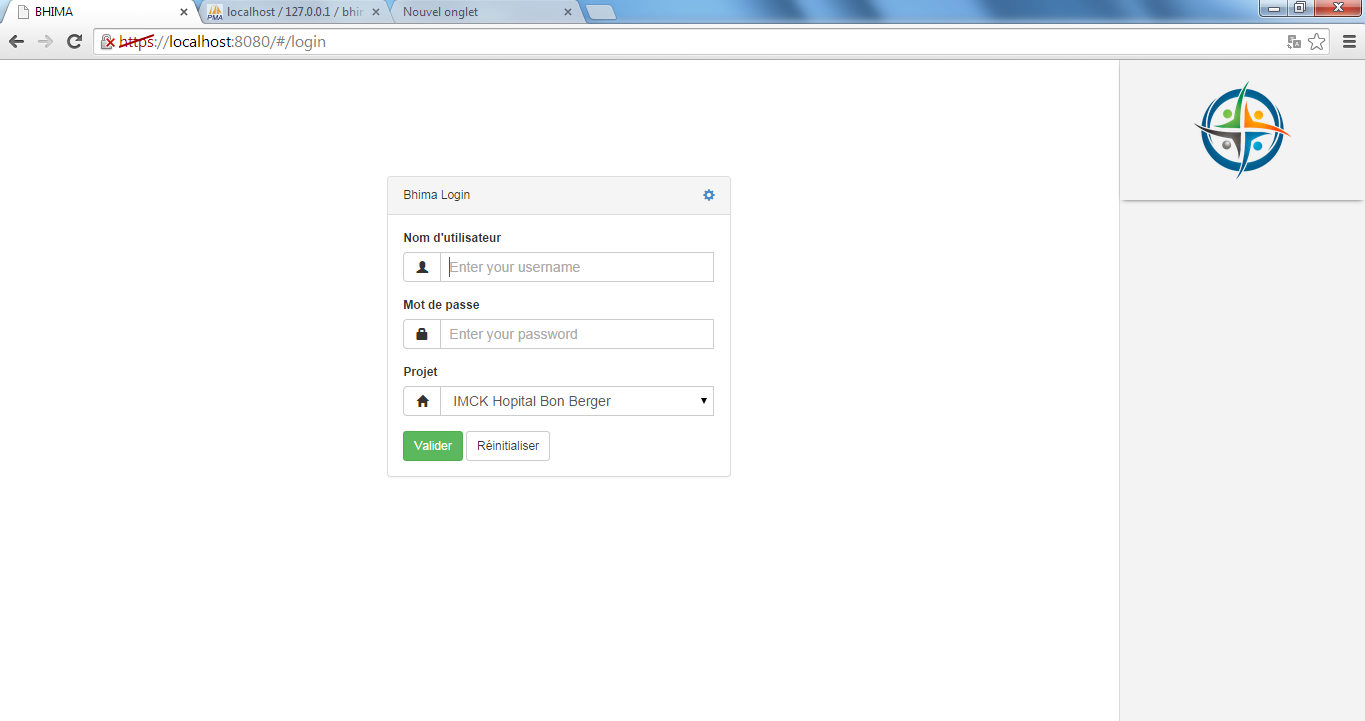
\includegraphics[width=12cm]{pic/login.png}
\end{center}
\caption{Page d'identification et authentification des utilisateurs}
\label{Page d'identification et authentification des utilisateurs}
\end{figure}
\\ L'accès au système n'est garanti que pour ceux qui possèdent un compte utilisateur, si l'utilisateur est authentifié alors il sera dirigé vers l'interface principale de l'application qui se présente de la manière suivante.
\newpage
\begin{figure}[h]
\begin{center}
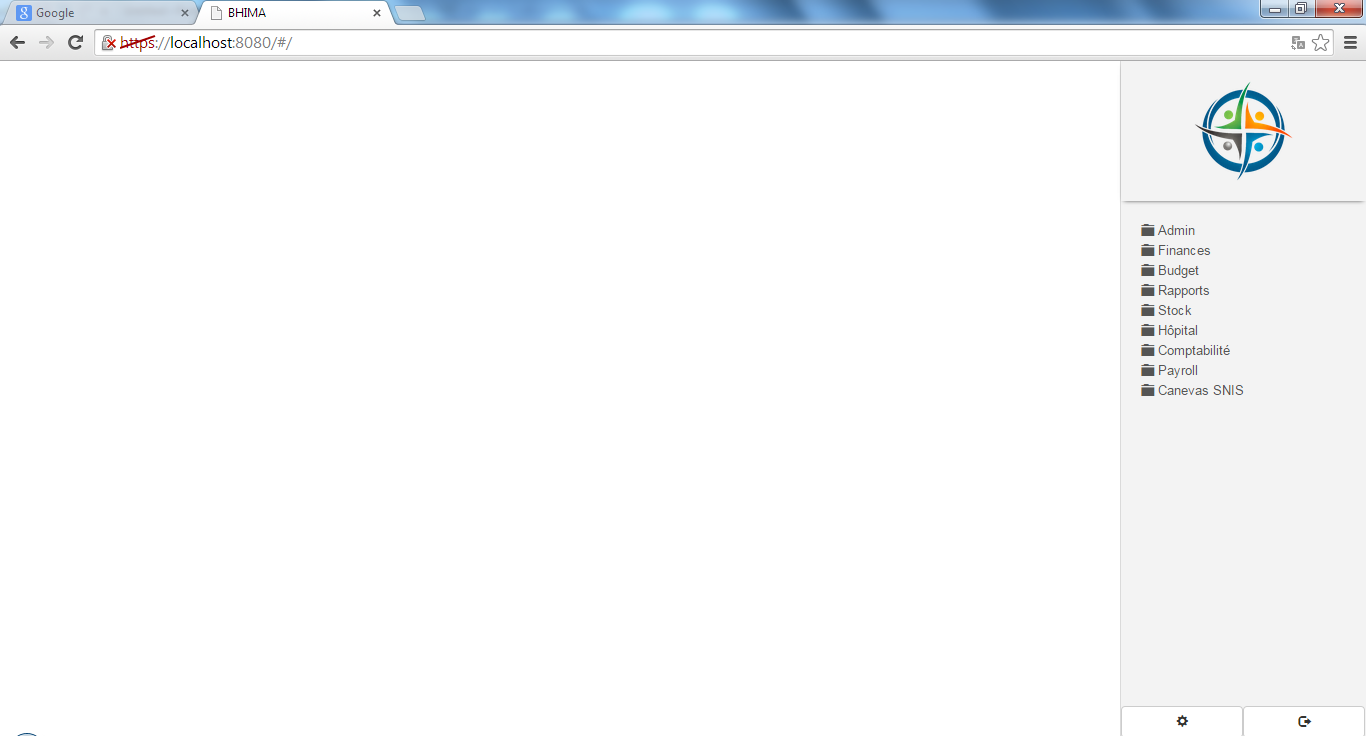
\includegraphics[width=10cm]{pic/mainInterface.png}
\end{center}
\caption{Interface principale de l'application}
\label{Interface principale de l'application}
\end{figure} 
Dans sa partie gauche de la figure ci-dessous on retrouve le logo IMA World Heath Ainsi que l'arborescence qui représente le niveau d'accès de l'utilisateur. En dessous de l'arborescence figure deux boutons, le premier 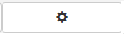
\includegraphics[scale=0.5]{pic/lang.png} permet de changer de langue et le second 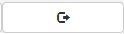
\includegraphics[scale=0.5]{pic/logout.png} permet de ce déconnecté du système.

\begin{figure}[h]
\begin{center}
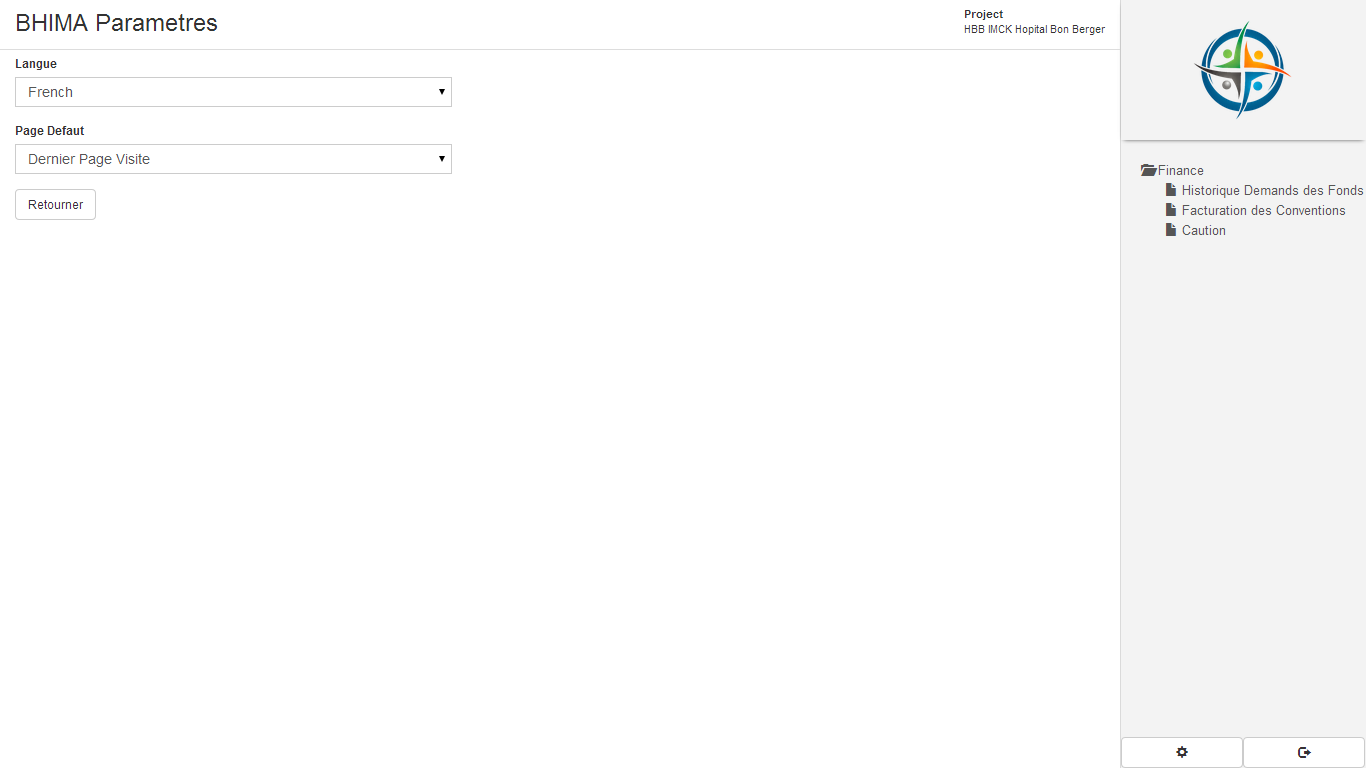
\includegraphics[width=10cm]{pic/changeLang.png}
\end{center}
\caption{Interface principale pour le changement de langue}
\label{Interface principale pour le changement de langue}
\end{figure} 
\newpage
\section{Les modules du système HMS}
Le système d'information HMS possède plusieurs modules qui sont représenté par l'arborescence ci-dessous.
\begin{figure}[h]
\begin{center}
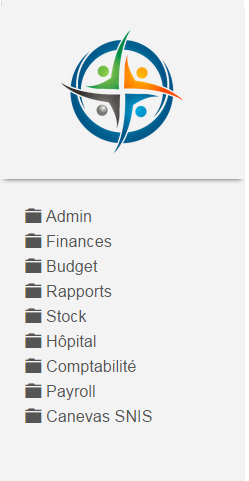
\includegraphics[width=4.5cm]{pic/arbo.png}
\end{center}
\caption{Arborescence du système}
\label{Arborescence du système}
Voici les différentes rubriques qui existent dans le système:
\end{figure} 
% Liste des modules
\begin{itemize}
\item Admin. %•
\item Finance
\item Budget
\item Rapports
\item Stock
\item Hôpital
\item Payroll
\item Comptabilité
\item Canevas SNIS
\end{itemize}
Nous allons à présent détailler chacun d'entre eux.
\newpage
%%%%%%%%%%%%%%%%%%%%%%%%%%%%%%%%%%%%%%%%%%%%%
%   MODULES DU SYSTEMES                     %
%%%%%%%%%%%%%%%%%%%%%%%%%%%%%%%%%%%%%%%%%%%%%
    
\chapter{Le module Admin}        
%////////////////////////////////////////////////%
% MODULE ADMIN
\section{Localisation}
Gestions Emplacement permet d'enregistrer toutes les localisations possible pour l'enregistrement des patients. L'interface principale se présente comme de la manière suivante.

\begin{figure}[h]
\begin{center}
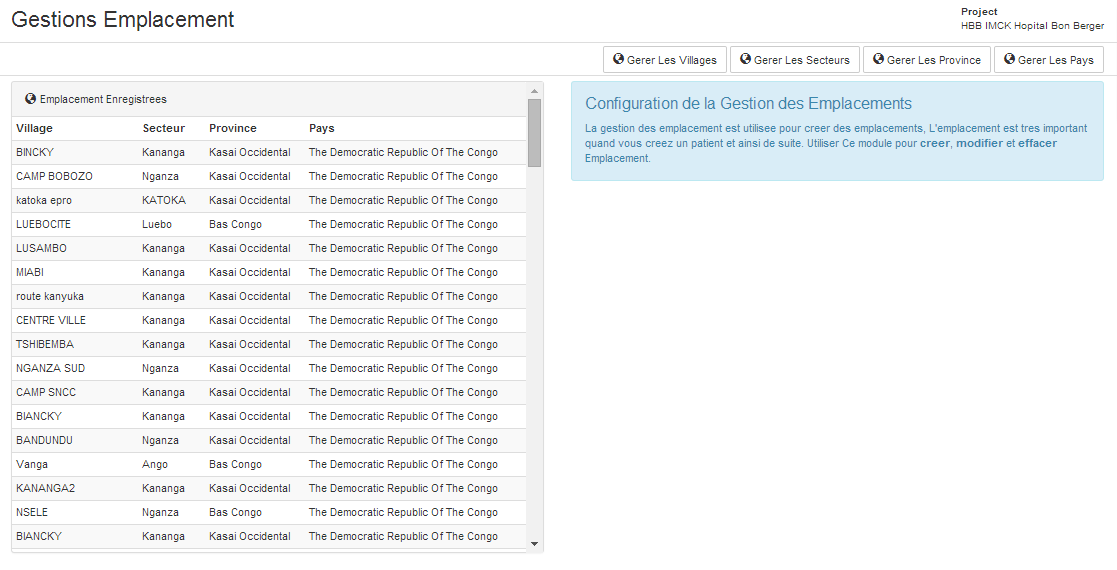
\includegraphics[width=14cm]{pic/AdminLocalisation.png}
\end{center}
\caption{Interface principale du module gestion des emplacement}
\label{Interface principale du module gestion des emplacement}
\end{figure}

Dans la partie droite l'on trouve le bouton qui permet d'ajouter les différents niveaux d'emplacement en commençant par la gestion des villages, des secteurs, des provinces ainsi que celui des pays. En dessous de ce menu de configuration est affiché sur un tableau les différents emplacements qui ont étaient enregistrés dans ce système. 
\newpage
\subsection{Gestion des villages}
Pour faire l'administration des villages, il suffit de cliquer sur le bouton\\ 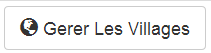
\includegraphics[scale=0.7]{pic/GererVillage.png}, ceci redirige vers la page qui permet une telle administration.

\begin{figure}[h]
\begin{center}
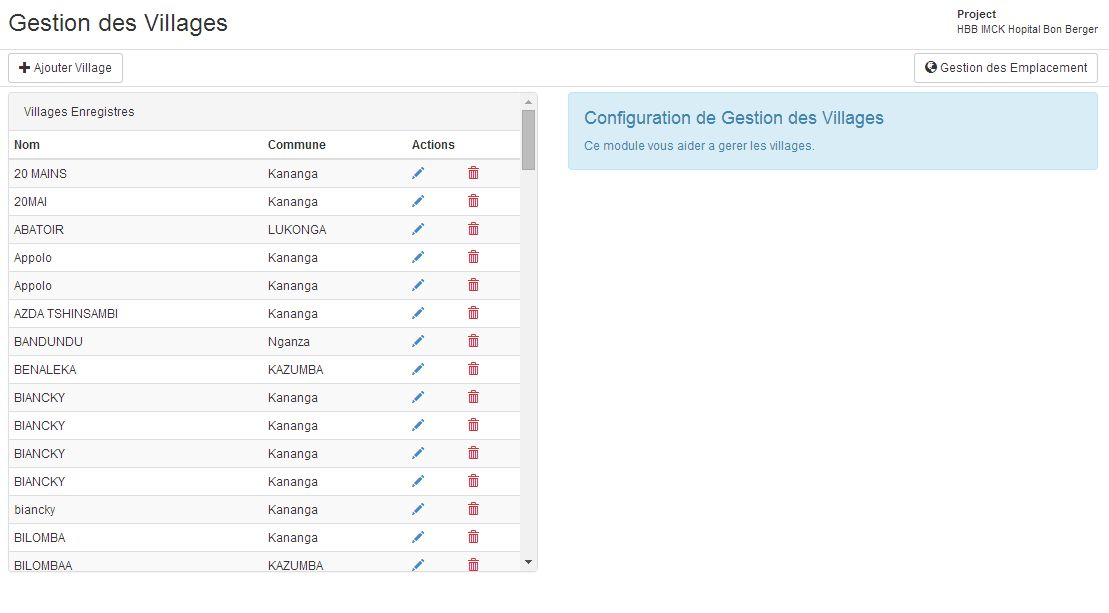
\includegraphics[width=14cm]{pic/AdminVillage.png}
\end{center}
\caption{Interface principale permettant d'administrer les villages}
\label{Interface principale permettant d'administrer les villages}
\end{figure}

Le bouton 
\includegraphics[scale=0.7]{pic/GestionEmplacement.png} redirige vers la page principale de la gestion des emplacements.

Le bouton 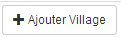
\includegraphics[scale=0.7]{pic/AddVillage.png} permet d'ajouter un village dans ladite liste.

\begin{figure}[h]
\begin{center}
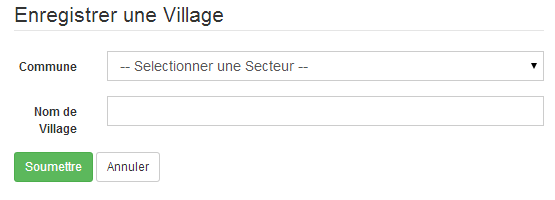
\includegraphics[width=14cm]{pic/FormAddVillage.png}
\end{center}
\caption{Formulaire permettant d'ajouter un village}
\label{Formulaire permettant d'ajouter un village}
\end{figure}

Le formulaire ci-haut apparait lorsqu'un utilisateur clique sur le bouton \textbf{ajouter village}. Ce formulaire possède deux champs, le premier \textbf{commune} renferme la liste de toutes les communes enregistré dans le système. 
L'enregistrement est effectif seulement si l'utilisateur clique sur le bouton soumettre. La liste des villages apparait sous forme de tableau. Ce tableau a trois rubriques. Le premier \textbf{Nom} renseigne sur le nom du village, le second \textbf{Commune} permet de savoir dans quelle commune se trouve le village et le dernier \textbf{Actions} renferme deux icônes le premier 
\includegraphics[scale=0.7]{pic/EditUser.png}  permet de modifier les informations sur un village et le second 
\includegraphics[scale=0.7]{pic/DeleteWRed.png}  permet de supprimer un village.

\subsection{Gérer les secteurs}
Pour faire l'administration des secteurs, il suffit de cliquer sur le bouton 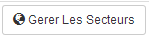
\includegraphics[scale=0.7]{pic/AdminSecteur.png} pour être redirigé vers la page qui permet une telle administration.

\begin{figure}[h]
\begin{center}
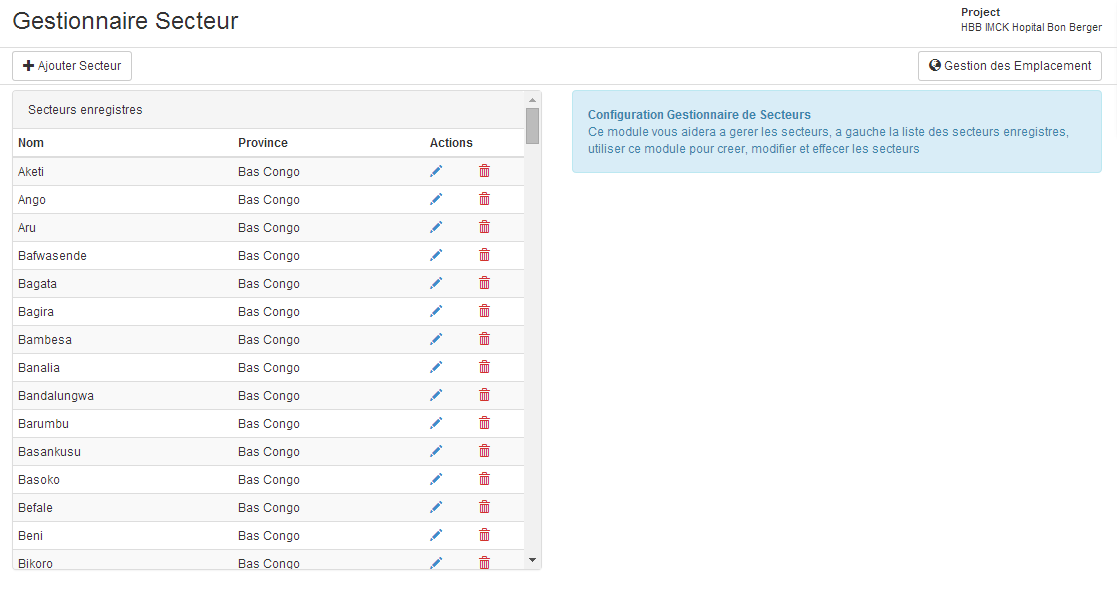
\includegraphics[width=14cm]{pic/FormulaireGestionSecteur.png}
\end{center}
\caption{Aperçue du plan Comptable}
\label{Aperçue du plan Comptable}
\end{figure}

Le bouton 
\includegraphics[scale=0.7]{pic/GestionEmplacement.png} redirige vers la page principale de la gestion des emplacements.
Le bouton 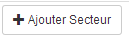
\includegraphics[scale=0.7]{pic/AddSecteur.png} permet d'ajouter un secteur dans ladite liste.

\begin{figure}[h]
\begin{center}
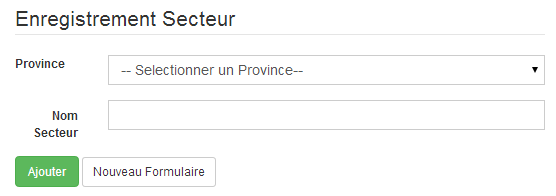
\includegraphics[width=14cm]{pic/FormAddSecteur.png}
\end{center}
\caption{Formulaire permettant d'ajouter les secteurs}
\label{Formulaire permettant d'ajouter les secteurs}
\end{figure}

Le formulaire ci-haut apparait lorsqu'un utilisateur clique sur le bouton \textbf{ajouter secteur}. Ce formulaire possède deux champs, le premier \textbf{Province} renferme la liste de toutes les provinces enregistré dans le système. 
L'enregistrement est effectif seulement si l'utilisateur clique sur le bouton Ajouter. La liste des secteurs apparait sous forme de tableau. Ce tableau a trois rubriques. Le premier\textbf{ Nom} renseigne sur le nom du secteur, le second \textbf{Province} permet de savoir dans quelle commune se trouve le village et le dernier \textbf{Actions} renferme deux icônes le premier 

\includegraphics[scale=0.7]{pic/EditUser.png}  permet de modifier les informations sur un secteur et le second 
 
\includegraphics[scale=0.7]{pic/DeleteWRed.png}  permet de supprimer un secteur.
\subsection{Gérer les provinces}
Pour faire l'administration des provinces, il suffit de cliquer sur le bouton 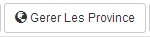
\includegraphics[scale=0.7]{pic/AdminProvince.png} pour être redigé vers la page qui permet une telle administration.
\begin{figure}[h]
\begin{center}
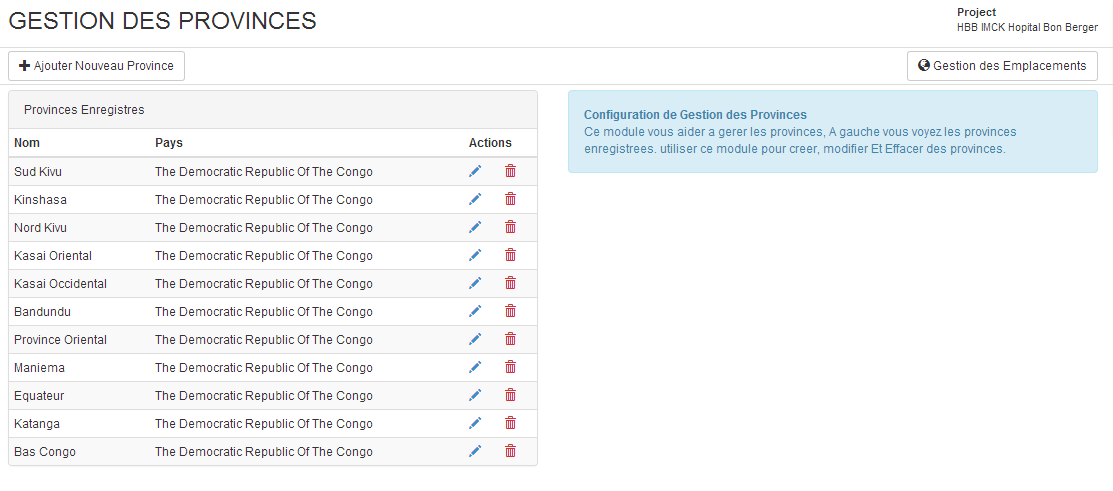
\includegraphics[width=14cm]{pic/InterfaceGestionProvince.png}
\end{center}
\caption{Interface principale permettant la gestion des provinces}
\label{Aperçue du plan Comptable}
\end{figure}

Le bouton 
\includegraphics[scale=0.7]{pic/GestionEmplacement.png} redirige vers la page principale de la gestion des emplacements.

Le bouton 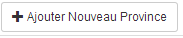
\includegraphics[scale=0.7]{pic/AddNewProvince.png} permet d'ajouter une province dans ladite liste.
\newpage
\begin{figure}[h]
\begin{center}
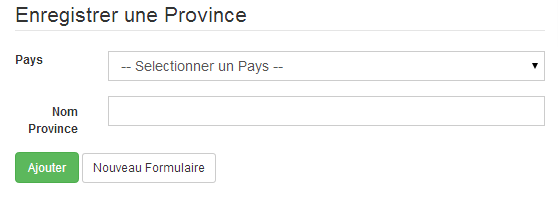
\includegraphics[width=14cm]{pic/FormNewProvince.png}
\end{center}
\caption{Formulaire permettant d'ajouter une province}
\label{Formulaire permettant d'ajouter une province}
\end{figure}


Le formulaire ci-haut apparait lorsqu'un utilisateur clique sur le bouton ajouter province. Ce formulaire possède deux champs, le premier Pays renferme la liste de tous les pays. 
L'enregistrement est effectif seulement si l'utilisateur clique sur le bouton Ajouter. La liste des provinces apparait sous forme de tableau. Ce tableau a trois rubriques. Le premier \textbf{Nom} renseigne sur le nom de la province, le second \textbf{Pays} permet de savoir dans quelle pays se trouve une province et le dernier \textbf{Actions} renferme deux icônes le premier 

\includegraphics[scale=0.7]{pic/EditUser.png}  permet de modifier les informations sur une province et le second  
\includegraphics[scale=0.7]{pic/DeleteWRed.png}  permet de supprimer une province.
\subsection{Gérer les pays}
Pour faire l'administration des pays, il suffit de cliquer sur le bouton 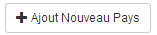
\includegraphics[scale=0.7]{pic/AddNewCountry.png}, ceci redirige vers la page qui permet une telle administration.
\begin{figure}[h]
\begin{center}
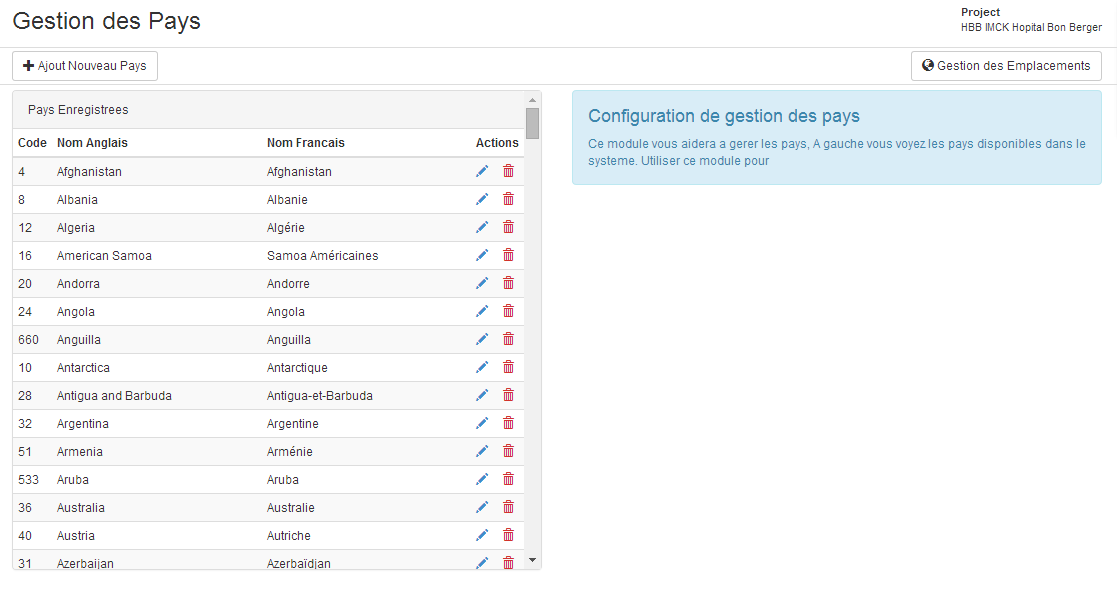
\includegraphics[width=14cm]{pic/AdminCountry.png}
\end{center}
\caption{Interface principale permettant la gestion des pays}
\label{Interface principale permettant la gestion des pays}
\end{figure}

Le bouton 
\includegraphics[scale=0.7]{pic/GestionEmplacement.png}  permet redirige vers la page principale de la gestion des emplacements.

Le bouton 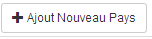
\includegraphics[scale=0.7]{pic/AddCountry.png} permet d'ajouter un pays dans ladite liste.

\begin{figure}[h]
\begin{center}
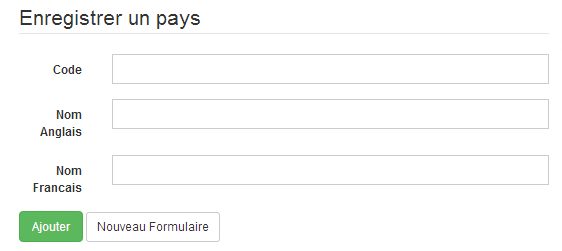
\includegraphics[width=16cm]{pic/SaveCountry.png}
\end{center}
\caption{Enregistrer un pays}
\label{Enregistrer un pays}
\end{figure}

Le formulaire ci-haut apparait lorsqu'un utilisateur clique sur le bouton \textbf{ajouter Nouveau pays}. Ce formulaire possède trois champs, le premier \textbf{Code} permet de donner un code à un pays ensuite un champ pour donner le nom du pays en \textbf{Anglais} et l'autre pour le \textbf{Français}.
L'enregistrement est effectif seulement si l'utilisateur clique sur le bouton Ajouter. La liste des pays apparait sous forme de tableau. Ce tableau a trois rubriques. Le premier \textbf{Code} renseigne sur le code qui a été attribué au pays, le second \textbf{Nom en anglais} suivi de \textbf{Nom}  et le dernier \textbf{Actions} renferme deux icônes le premier 
\includegraphics[scale=0.7]{pic/EditUser.png}  permet de modifier les informations sur un pays et le second 
\includegraphics[scale=0.7]{pic/DeleteWRed.png}  permet de supprimer un pays.



\newpage
\chapter{Le module Rapports}        
%////////////////////////////////////////////////%
Le module rapports permet de pouvoir visualiser plusieurs types des rapports résultants du fonctionnements du système, La figure ci-dessous représente avec exactitude ce module avec les différents sous éléments.

\begin{figure}[h]
\begin{center}
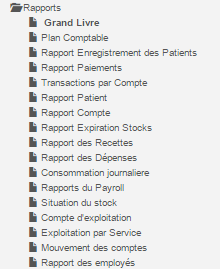
\includegraphics[width=4cm]{pic/ArboReport.png}
\end{center}
\caption{Arborescence du module Rapports}
\label{Arborescence du module Rapports}
\end{figure}
\newpage
\section{Rapport Enregistrement des Patients}
Le rapport d'enregistrement des patients permet de visualiser l'historique d'enregistremet des patients dans le système. L'interface principale permettant de voire le rapport d'enregistrement des patients se présente de la manière suivante. 

\begin{figure}[h]
\begin{center}
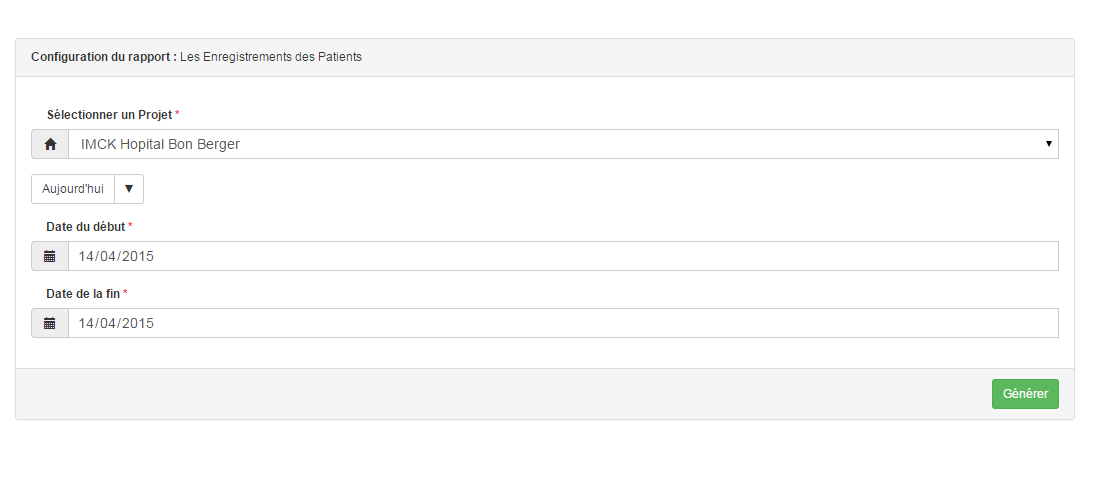
\includegraphics[width=10cm]{pic/RapportEnrPatient.png}
\end{center}
\caption{Aperçue de l'interface principale du rapport d'enregistrement des patients}
\label{Aperçue de l'interface principale du rapport d'enregistrement des patients}
\end{figure}

Par défaut le rapport d'enregistrement des patients affiche la liste des patients enregistrés le jour courant, l'interface du rapport d'enregistrement dispose de plusieurs outils permettant de visualiser les anciennes données enregistrés.

Le bouton 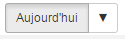
\includegraphics[scale=0.7]{pic/Todays.png} donne la possibilité de visualiser les enregistrements du jour courant, de la semaine courante mais aussi ceux du mois courant. 

Il existe aussi  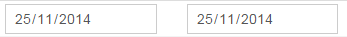
\includegraphics[scale=0.7]{pic/PlageTimes.png} qui permet visualiser le rapport d'enregistrement en precisant une plage de valeur entre deux dates.

Le bouton 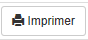
\includegraphics[scale=0.7]{pic/Print.png} permet d'imprimer le rapport d'enregistrement des patients

Il existe aussi une liste de choix qui donne la possibilité de visualiser le rapport d'enregistrement par projets ou bien de tous le projet à la fois.

En bas de page on retrouve les indicateurs sur le résultat de la recherche permettant de connaitre le nombre des patients trouvés  ainsi que la repartion par sexe. 

\begin{figure}[h]
\begin{center}
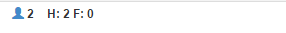
\includegraphics[width=5cm]{pic/IndicRecherche.png}
\end{center}
\caption{Aperçue des indicateurs sur le résultat de la recherche}
\label{Aperçue des indicateurs sur le résultat de la recherche}
\end{figure}



%////////////////////////////////////////////////%
\newpage
\chapter{Hôpital}        

Le module Hôpital est composé des sous modules qui permettent d'administrer les patients. La figure ci-dessous représente avec exactitude ce module avec ses différents sous éléments.

\begin{figure}[h]
\begin{center}
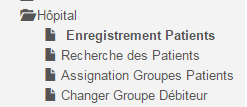
\includegraphics[width=6cm]{pic/HopitalArbo.png}
\end{center}
\caption{Arborescence du module Hôpital}
\label{Arborescence du module Hôpital}
\end{figure}

\section{Enregistrement des Patients}
Le module permttant l'enregistrement de patient permet d'enregistrer les patients dans le système, lors de toute opération d'enregistrement il est nécessaire de pouvoir spécifier dans quelle circonstance se derroule l'enregistrement, il peut s'agir d'un nouveau patient à l'hôpital, mais aussi des patients qui ont été enregistrés, et ont une histoire prescription / vente avec l'hôpital, mais n'ont jamais été enregistrée dans le système BHIMA et dans le dernier cas pour le patient qui existe déjà dans le système. 

Le formulaire permettant l'enregistrement des patients dans le système est subdivisé en quatres parties, la prémière partie se présente de la manière suivante.

\begin{figure}[h]
\begin{center}
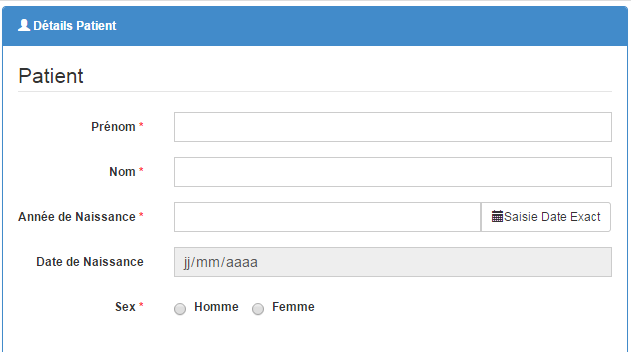
\includegraphics[width=12cm]{pic/DetailPatient.png}
\end{center}
\caption{Aperçue de la partie Détail Patient}
\label{Aperçue de la partie Détail Patient}
\end{figure}

Dans cette prémière partie il est nécessaire de fournir les informations liés au Prénom ainsi que le nom du patient, sa date de naissance ainsi que le sexe du patient.

La seconde partie est reservée à l'emplacement du patient, pour cela il est nécessaire de pouvoir renseigner l'emplacement origin mais aussi l'emplacement dans la quelle se trouve présentement le patient, voici un apperçue du module qui permet de sélectionner l'emplacement origine et présent d'un patient.

\begin{figure}[h]
\begin{center}
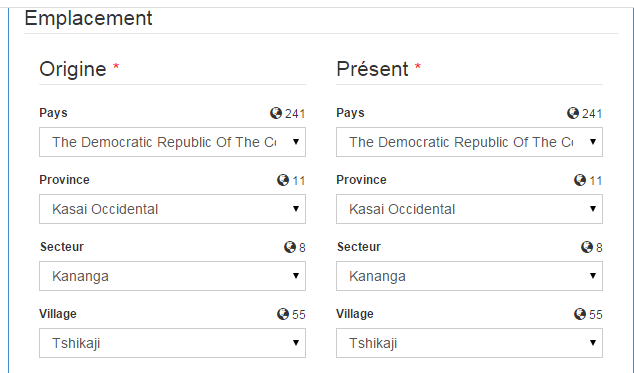
\includegraphics[width=12cm]{pic/EmplacementPatient.png}
\end{center}
\caption{Aperçue de l'interface liée à l'emplacement d'un patient}
\label{Aperçue de l'interface liée à l'emplacement d'un patient}
\end{figure}

Il est nécessaire de pouvoir fournir les informations liées au pays du patient, sa province, son secteur, ainsi que son village d'origine en plus de cela il faudrait aussi preciser l'emplacement présent du patient.
\newpage
La troisième partie consacré à la finance permet d'attribué un groupe débiteur à un patient, pour le patient qui n'appartienne pas à une convention sont généralement enregistrés comme étant des patients payants cash. mais si non il faudrait les attribuer à des bons groupes débiteurs. Voici l'apperçue du formulaire permettant l'attribution des patients à des groupes débiteurs.

\begin{figure}[h]
\begin{center}
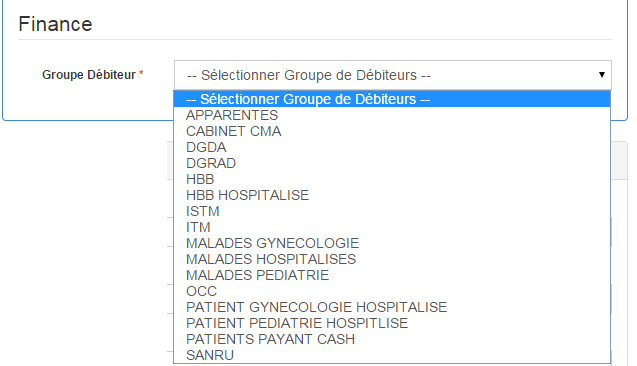
\includegraphics[width=7cm]{pic/SelectGrDebiteur.png}
\end{center}
\caption{Aperçue de l'interface permettant la sélection d'un groupe débiteur}
\label{Aperçue de l'interface permettant la sélection d'un groupe débiteur}
\end{figure} 
 
La quatrième partie permet concerne les informations optionnelles, liés à un patient il s'agit du numéro de téléphone, l'adresse e-mail, la rue, le nom du pére, de la mère, la religion, Etat civil, la profession, etc...
Voici l'apperçue du formulaire qui permet de permet de renseigner ses informations optionnelles.

\begin{figure}[h]
\begin{center}
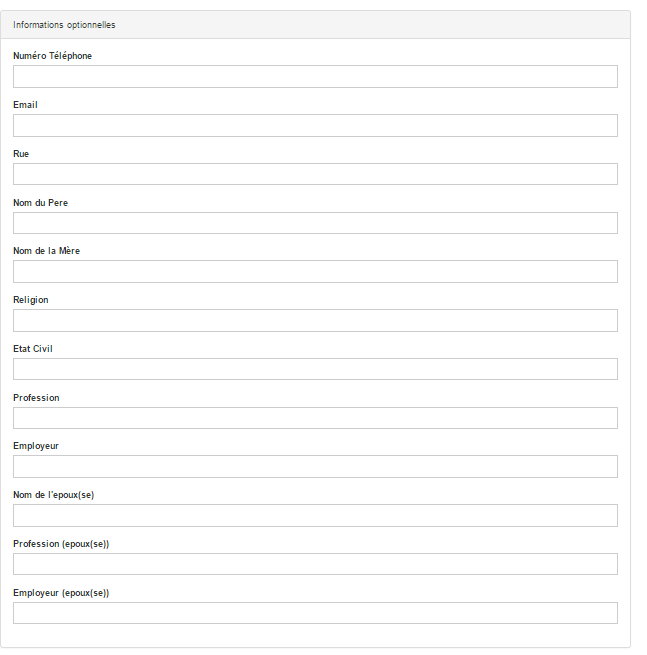
\includegraphics[width=8cm]{pic/InfoOptionnel.png}
\end{center}
\caption{Aperçue de l'interface permettant l'engistrement des informations optionnelles}
\label{Aperçue de l'interface permettant l'engistrement des informations optionnelles}
\end{figure} 
Dans la partie droite du formulaire on la zone permettant de preciser le type d'enregistrement, à l'exception des deux premières options la troisième permet de rechercher les informations liées aux patients. voici comment se présente l'interface permettant de préciser le type d'enregistrement à appliquer lors de l'enregistrement d'un patient. 

Et une fois qu'on a choisi l'option d'enregistrement, il suffit de cliquer sur le bouton 
\includegraphics[scale=0.7]{pic/EnregPatient.png} pour rendre effective l'enregistrement du patient dans le système.

\begin{figure}[h]
\begin{center}
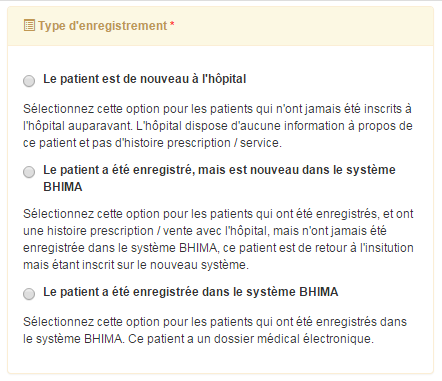
\includegraphics[width=8cm]{pic/TypeEnregistrement.png}
\end{center}
\caption{Aperçue de l'interface permettant de préciser le type d'enregistrement}
\label{Aperçue de l'interface permettant de préciser le type d'enregistrement}
\end{figure}  
\newpage
Lorsqu'on coche sur la dernière option, l'interface d'enregistrement change d'apparence et la zone permettant de rechercher un patient apparait avec la possibilité de rechercher un patient soit par le \textbf{ID débiteur} ou bien par \textbf{le nom du malade}. La figure ci-dessous illustre la recherche d'un patient déjà enregistré dans le système.

\begin{figure}[h]
\begin{center}
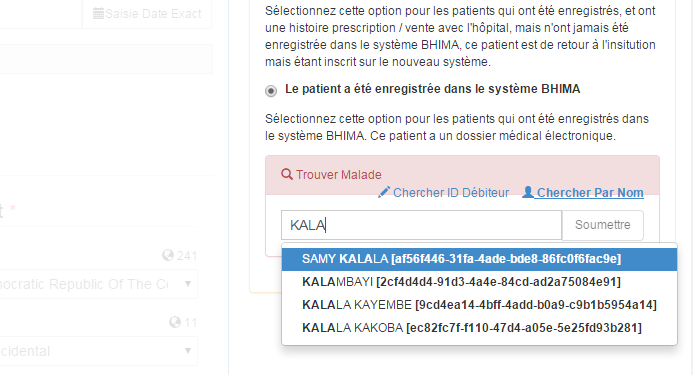
\includegraphics[width=8cm]{pic/ApRecherche.png}
\end{center}
\caption{Aperçue de l'interface permettant la recherche d'un patient déjà enregistré}
\label{Aperçue de l'interface permettant la recherche d'un patient déjà enregistré}
\end{figure}  

Et si l'on clique sur le bouton \textbf{Soumettre pour que s'affiche les informations liées au patient}

\newpage
\section{Recherche des patients}
Le module recherche des patients, permet de faire des recherches détaillées par rapport aux informations liées à des patients, le système permet de pouvoir faire la recherche en se basant soit par le nom, le prénom, l'année de naissance ainsi que le sexe.

\begin{figure}[h]
\begin{center}
\includegraphics[width=11cm]{pic/recherchePatient.png}
\end{center}
\caption{Aperçue de l'interface permettant la recherche détaillées des patients}
\label{Aperçue de l'interface permettant la recherche détaillées des patients}
\end{figure}  

Pour pouvoir lancer la recherche il suffit de cliquer sur le bouton \includegraphics[scale=0.7]{pic/ExeButton.png}

Il est possible de pouvoir rechercher les patients en incluant la localisation géographique des patients dans la recherche grâce au bouton \includegraphics[scale=0.7]{pic/LocalisationRecherche.png}

\subsection{Illustration de la recheche détaillée}
Supposons qu'on a besoin de rechercher les femmes qui sont nées en 1960. il suffirait de remplir la fiche de la manière suivante, et appuiyer sur le bouton Exécuter pour que s'affiche en dessous du formulaire les résultats de la recherche. 

\begin{figure}[h]
\begin{center}
\includegraphics[width=11cm]{pic/RechecheDetailler.png}
\end{center}
\caption{Aperçue de l'interface permettant de visualiser les résultats de la recherche}
\label{Aperçue de l'interface permettant de visualiser les résultats de la recherche}
\end{figure} 

\subsection{Illustration de la recheche détaillée incluant la localisation géographique}
Supposont cette fois ci qu'on aimerai connaitre combien y a t'il des femmes qui sont né en 1992 et qui habitent dans le village de TSHIKAJI.

\begin{figure}[h]
\begin{center}
\includegraphics[width=11cm]{pic/RechercheDetGeo.png}
\end{center}
\caption{Aperçue d'une recherche incluant la localisation géographique}
\label{Aperçue d'une recherche incluant la localisation géographique}
\end{figure} 
 
\newpage
\section{Assignations groupes débiteurs}
Permet d'assigné un patient dans des groupes débiteurs qui bénéficie des certaines avantages pendant le processus de la vente et de la facturation des malades.

Pour assigner un patient à un groupe, il faudrait prémièrement le rechercher et en suite cocher dans les différentes assignations qu'il lui faut en suite clique sur le bouton \textbf{Sauver changement}

Voici comment se compose l'interface principale de ce module.

\begin{figure}[h]
\begin{center}
\includegraphics[width=11cm]{pic/AssPatients.png}
\end{center}
\caption{Aperçue de l'interface permettant de rechercher un patient}
\label{Aperçue de l'interface permettant de rechercher un patient}
\end{figure} 

Après avoir rechercher un patient, il suffit juste de cliquer sur le bouton soumettre pour qu'apparaise l'interface permettant de chocher les différents assignations nécessaire.

\begin{figure}[h]
\begin{center}
\includegraphics[width=11cm]{pic/AssiGames.png}
\end{center}
\caption{Aperçue de l'interface permettant l'assignations à des groupes des patients}
\label{Aperçue de l'interface permettant l'assignations à des groupes des patients}
\end{figure} 

Si l'on a choisi un patient mais qu'on aimerai choisir un autre il suffit de cliquer sur le bouton \includegraphics[scale=0.7]{pic/ComeBack.png}  pour revenir à l'interface permettant de rechercher un patient.

Si l'on veut aussi modifier l'assignation d'un patient à un groupe, il suffit de suivre le même procedure que pour l'assignation mais dans ce cas, les groupes dans lesquelles a été assigné le patient seront coché en avance, une fois que les groupes ont été modifier, il suffit à nouveau de cliquer sur le bouton \includegraphics[scale=0.7]{pic/SaveChang.png} pour pouvoir enregistrer les changements.

\section{Changer groupe débiteur}
Le module changer le groupe débiteur est en fait un module permettant l'affectation des patients à des groupes débiteurs, le processus d'affection des patients à des groupes débiteurs consiste premièrement à rechercher le patient et en suite à trouver dans quelle groupe le placer.

Voici l'interface principale permettant l'affectation des patients à des groupes débiteurs.

\begin{figure}[h]
\begin{center}
\includegraphics[width=11cm]{pic/AffeGrDeb.png}
\end{center}
\caption{Aperçue de l'interface permettant l'affectation d'un patient à un groupe créditeur}
\label{Aperçue de l'interface permettant l'affectation d'un patient à un groupe créditeur}
\end{figure}

\newpage
Une fois qu'un débiteur a été trouver, l'interface d'utilisation change et dans sa prémière partie, fourni les informations liées à un patient et dans la séconde partie apparait la liste des groupes débiteurs existant au sein dans le système, et si le patient appartient déjà à un groupe débiteur ce dernier sera directement sélectionner par défaut.

Si le choix du groupe débiteur est fait, il suffit maintenant de cliquer sur le bouton \textbf{Soumettre} pour pouvoir confirmer l'affection d'un patient à un groupe débiteur, ce module est utilisé dans la plupart des temps si l'on veut modifier le groupe débiteur dans lequel appartient un patient.

\begin{figure}[h]
\begin{center}
\includegraphics[width=11cm]{pic/AffectGrDebiteur.png}
\end{center}
\caption{Aperçue du processus d'affectation}
\label{Aperçue du processus d'affectation}
\end{figure}

%%%%%%%%%%%%%%%%%%%%%%%%%%%%%%%%%%%%%%%%%%%%%%%%%
% Table des matieres
\tableofcontents
\end{document}